\section{Results}
\label{sec:results}

\subsection{Output Complexity Tracks Input Complexity}
\label{sec:complexity}

\Tabref{tab:complexity} presents the full results across all 14 complexity-graded prompts. Two patterns emerge clearly.

\para{Total information amplification.}
Output compressed bits consistently exceed input compressed bits, with the \infoamp ranging from $0.9\times$ (trivial fact) to $19.5\times$ (history explanation). Linear regression on total gzip bits yields slope $= 4.15$, $r^2 = 0.649$, $p = 5.08 \times 10^{-4}$, confirming that output information tracks input information.

\para{Density reduction.}
Despite the total amplification, the \densityratio is consistently below 1 for all but the shortest prompts. For prompts at Level 3 and above ($> 50$ bytes), the mean \densityratio is {\bf 0.49}, meaning each byte of output carries roughly half the information of each byte of input. Spearman correlation between input and output bpb (for texts $> 50$ bytes) is $\rho = 0.881$, $p = 3.11 \times 10^{-5}$.

The apparent paradox resolves via a simple decomposition:
\begin{equation}
    \text{Total info ratio} = \underbrace{\text{Length expansion}}_{{6\text{--}44\times}} \;\times\; \underbrace{\text{Density ratio}}_{{0.34\text{--}0.64\times}}.
    \label{eq:decomp}
\end{equation}
The model generates $6$--$44\times$ more text than the input, but each byte is less informationally dense. The ``extra'' total bits come from the model's weights---compressed training data---not from the input alone.

\begin{table}[t]
    \centering
    \caption{Input--output information metrics across complexity levels. \textbf{Density ratio} $< 1$ indicates the output is less informationally dense per byte than the input. Best (lowest) density ratios in \textbf{bold}.}
    \label{tab:complexity}
    \resizebox{\textwidth}{!}{%
    \begin{tabular}{@{}clrrrrrrr@{}}
        \toprule
        \textbf{Level} & \textbf{Prompt} & \textbf{In chars} & \textbf{Out chars} & \textbf{Length exp.} & \textbf{In bpb} & \textbf{Out bpb} & \textbf{Density ratio} & \textbf{Total info ratio} \\
        \midrule
        1 & trivial\_fact & 12 & 9 & 0.8$\times$ & 21.33 & 25.78 & 1.21 & 0.9$\times$ \\
        1 & single\_word & 10 & 34 & 3.4$\times$ & 24.00 & 12.71 & 0.53 & 1.8$\times$ \\
        1 & yes\_no & 16 & 289 & 18.1$\times$ & 18.00 & 5.51 & \textbf{0.31} & 5.5$\times$ \\
        \cmidrule(lr){1-9}
        2 & capital & 30 & 31 & 1.0$\times$ & 13.33 & 13.16 & 0.99 & 1.0$\times$ \\
        2 & definition & 38 & 180 & 4.7$\times$ & 12.00 & 6.44 & 0.54 & 2.5$\times$ \\
        2 & simple\_list & 26 & 51 & 2.0$\times$ & 14.15 & 11.14 & 0.79 & 1.5$\times$ \\
        \cmidrule(lr){1-9}
        3 & explain\_concept & 76 & 3,387 & 44.6$\times$ & 9.16 & 3.15 & \textbf{0.34} & 15.3$\times$ \\
        3 & compare & 114 & 3,017 & 26.5$\times$ & 7.93 & 3.26 & 0.41 & 10.9$\times$ \\
        3 & history & 113 & 4,974 & 44.0$\times$ & 7.79 & 3.45 & 0.44 & 19.5$\times$ \\
        \cmidrule(lr){1-9}
        4 & technical\_detail & 361 & 7,614 & 21.1$\times$ & 5.87 & 3.19 & 0.54 & 11.5$\times$ \\
        4 & analysis & 456 & 5,720 & 12.5$\times$ & 5.58 & 3.21 & 0.57 & 7.2$\times$ \\
        \cmidrule(lr){1-9}
        5 & data\_analysis & 624 & 4,237 & 6.8$\times$ & 4.74 & 2.68 & 0.56 & 3.8$\times$ \\
        5 & code\_generation & 497 & 8,535 & 17.2$\times$ & 5.18 & 1.91 & \textbf{0.37} & 6.3$\times$ \\
        \cmidrule(lr){1-9}
        6 & multi\_domain & 1,472 & 9,285 & 6.3$\times$ & 4.90 & 3.13 & 0.64 & 4.0$\times$ \\
        \bottomrule
    \end{tabular}
    }
\end{table}

\subsection{Gibberish Controls}
\label{sec:gibberish}

\Tabref{tab:gibberish} shows results for gibberish inputs. High-entropy inputs (\eg random ASCII at 9.60 bpb, keyboard mashing at 10.26 bpb) produce outputs with typical LLM density (${\sim}5$--$7$ bpb), not correspondingly high-information responses. The model produces explanatory or confused text acknowledging the nonsensical input.

The exception is revealing: repeated nonsense words compress extremely well (1.43 bpb due to repetition), but the model's response has normal density (7.68 bpb). This confirms that gzip bpb measures statistical regularity, not semantic content---and that the model does not ``amplify'' either kind.

\begin{table}[t]
    \centering
    \caption{Gibberish control experiment. High-entropy inputs do not produce high-information outputs. The model generates responses with typical LLM density regardless of input entropy.}
    \label{tab:gibberish}
    \begin{tabular}{@{}lrrl@{}}
        \toprule
        \textbf{Gibberish type} & \textbf{In bpb} & \textbf{Out bpb} & \textbf{Model behavior} \\
        \midrule
        Random ASCII (100) & 9.60 & 6.66 & Tries to interpret \\
        Random ASCII (500) & 6.66 & 6.74 & Similar density \\
        Shuffled words & 8.80 & 5.53 & Explains confusion \\
        Keyboard mash & 10.26 & 7.65 & Acknowledges nonsense \\
        Repeated nonsense & 1.43 & 7.68 & Normal response \\
        Unicode symbols & 8.65 & 4.34 & Describes symbols \\
        \bottomrule
    \end{tabular}
\end{table}

\subsection{Human vs.\ LLM Text Compression}
\label{sec:humanvsgpt}

On the \gptwiki corpus ($n = 99$ pairs, filtered to $\geq 100$ characters), we find that GPT-generated text is \emph{less} compressible by gzip than human text: mean bpb of $6.146 \pm 0.858$ vs.\ $5.133 \pm 0.888$ (Wilcoxon signed-rank $p = 2.33 \times 10^{-11}$, Cohen's $d = -1.161$).

This result directly \textbf{contradicts} \citet{wang2025lossless}, who report that LLM text is $20\times$ more compressible than human text. The key difference is the compressor: Wang et al.\ use an LLM as the compressor (arithmetic coding with an LLM prior), while we use gzip. LLM text follows the model's statistical patterns (predictable to LLMs) but has slightly higher surface-level entropy than human text (less predictable to statistical compressors like gzip). This finding demonstrates that \textbf{the choice of compressor is decisive} for conclusions about LLM text information content.

\subsection{LLM Log-Probability Analysis}
\label{sec:logprob}

\Tabref{tab:logprob} compares gzip-based and log-probability-based information measures. The contrast is stark: while gzip assigns outputs $360$--$18{,}016$ bits, the model's own log-probabilities assign only $0$--$551$ bits (excluding Level 4), corresponding to a mean of ${\sim}0.3$ \bpt.

\begin{table}[t]
    \centering
    \caption{Comparison of gzip and log-probability information measures. From the model's own perspective, outputs contain dramatically less information than gzip suggests. $^*$Level 4 anomaly likely reflects high uncertainty in economic analysis content.}
    \label{tab:logprob}
    \begin{tabular}{@{}clrrrr@{}}
        \toprule
        \textbf{Level} & \textbf{Prompt type} & \textbf{In (gzip bits)} & \textbf{Out (gzip bits)} & \textbf{Out (logprob bits)} & \textbf{Bits/token} \\
        \midrule
        1 & Trivial & 320 & 360 & 0 & 0.00 \\
        2 & Simple & 424 & 6,040 & 88 & 0.28 \\
        3 & Conceptual & 808 & 14,624 & 378 & 0.33 \\
        4 & Technical & 1,424 & 13,728 & 14,922 & 13.23$^*$ \\
        5 & Data analysis & 2,744 & 18,016 & 551 & 0.34 \\
        \bottomrule
    \end{tabular}
\end{table}

The $10$--$40\times$ gap between gzip bits and log-probability bits reveals that LLM outputs are far more predictable to an LLM than to a statistical compressor. The model's outputs lie on a low-dimensional manifold of its learned distribution---they are nearly deterministic given the prompt and the model's weights.

The Level 4 anomaly (13.23 \bpt) likely reflects a prompt requiring economic analysis, where the model faces genuine uncertainty among many plausible responses. This exception highlights that information content depends on how constrained the model's response space is.

\begin{figure}[t]
    \centering
    \begin{subfigure}[b]{0.48\textwidth}
        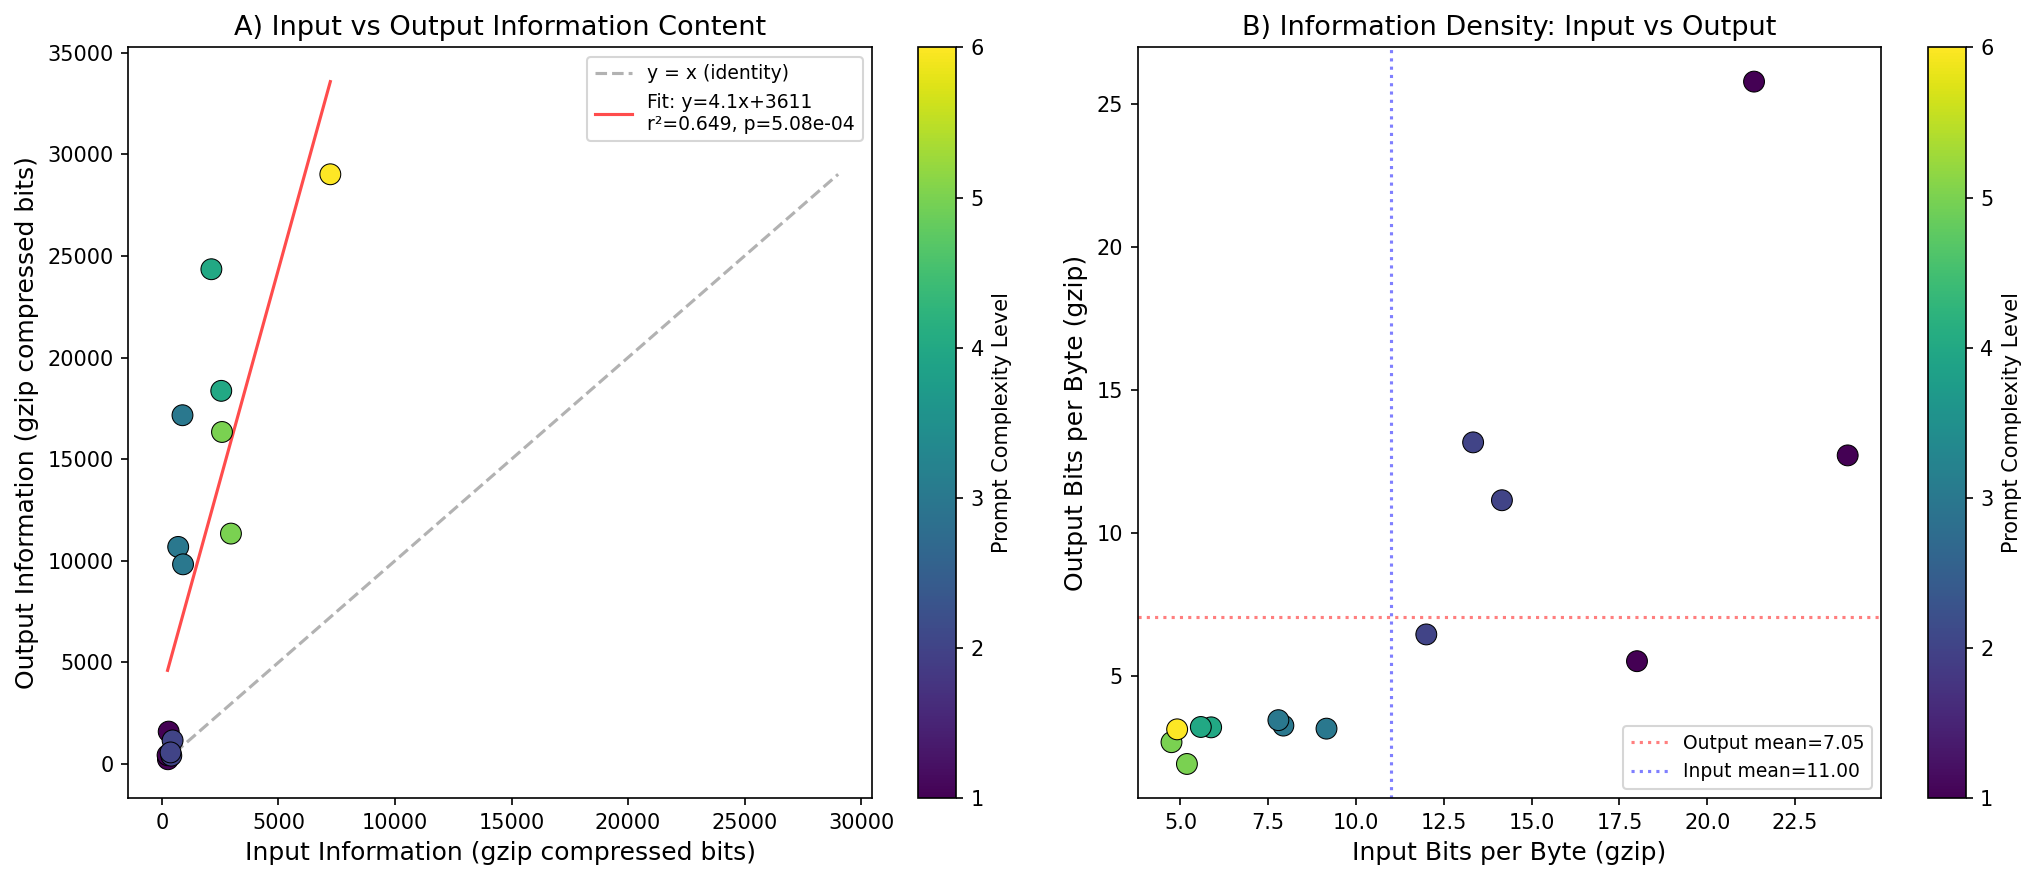
\includegraphics[width=\textwidth]{figures/fig1_input_vs_output_complexity.png}
        \caption{Input vs.\ output complexity (gzip bits). Output total bits exceed input bits, but the relationship is strongly linear ($r^2 = 0.649$).}
        \label{fig:complexity}
    \end{subfigure}
    \hfill
    \begin{subfigure}[b]{0.48\textwidth}
        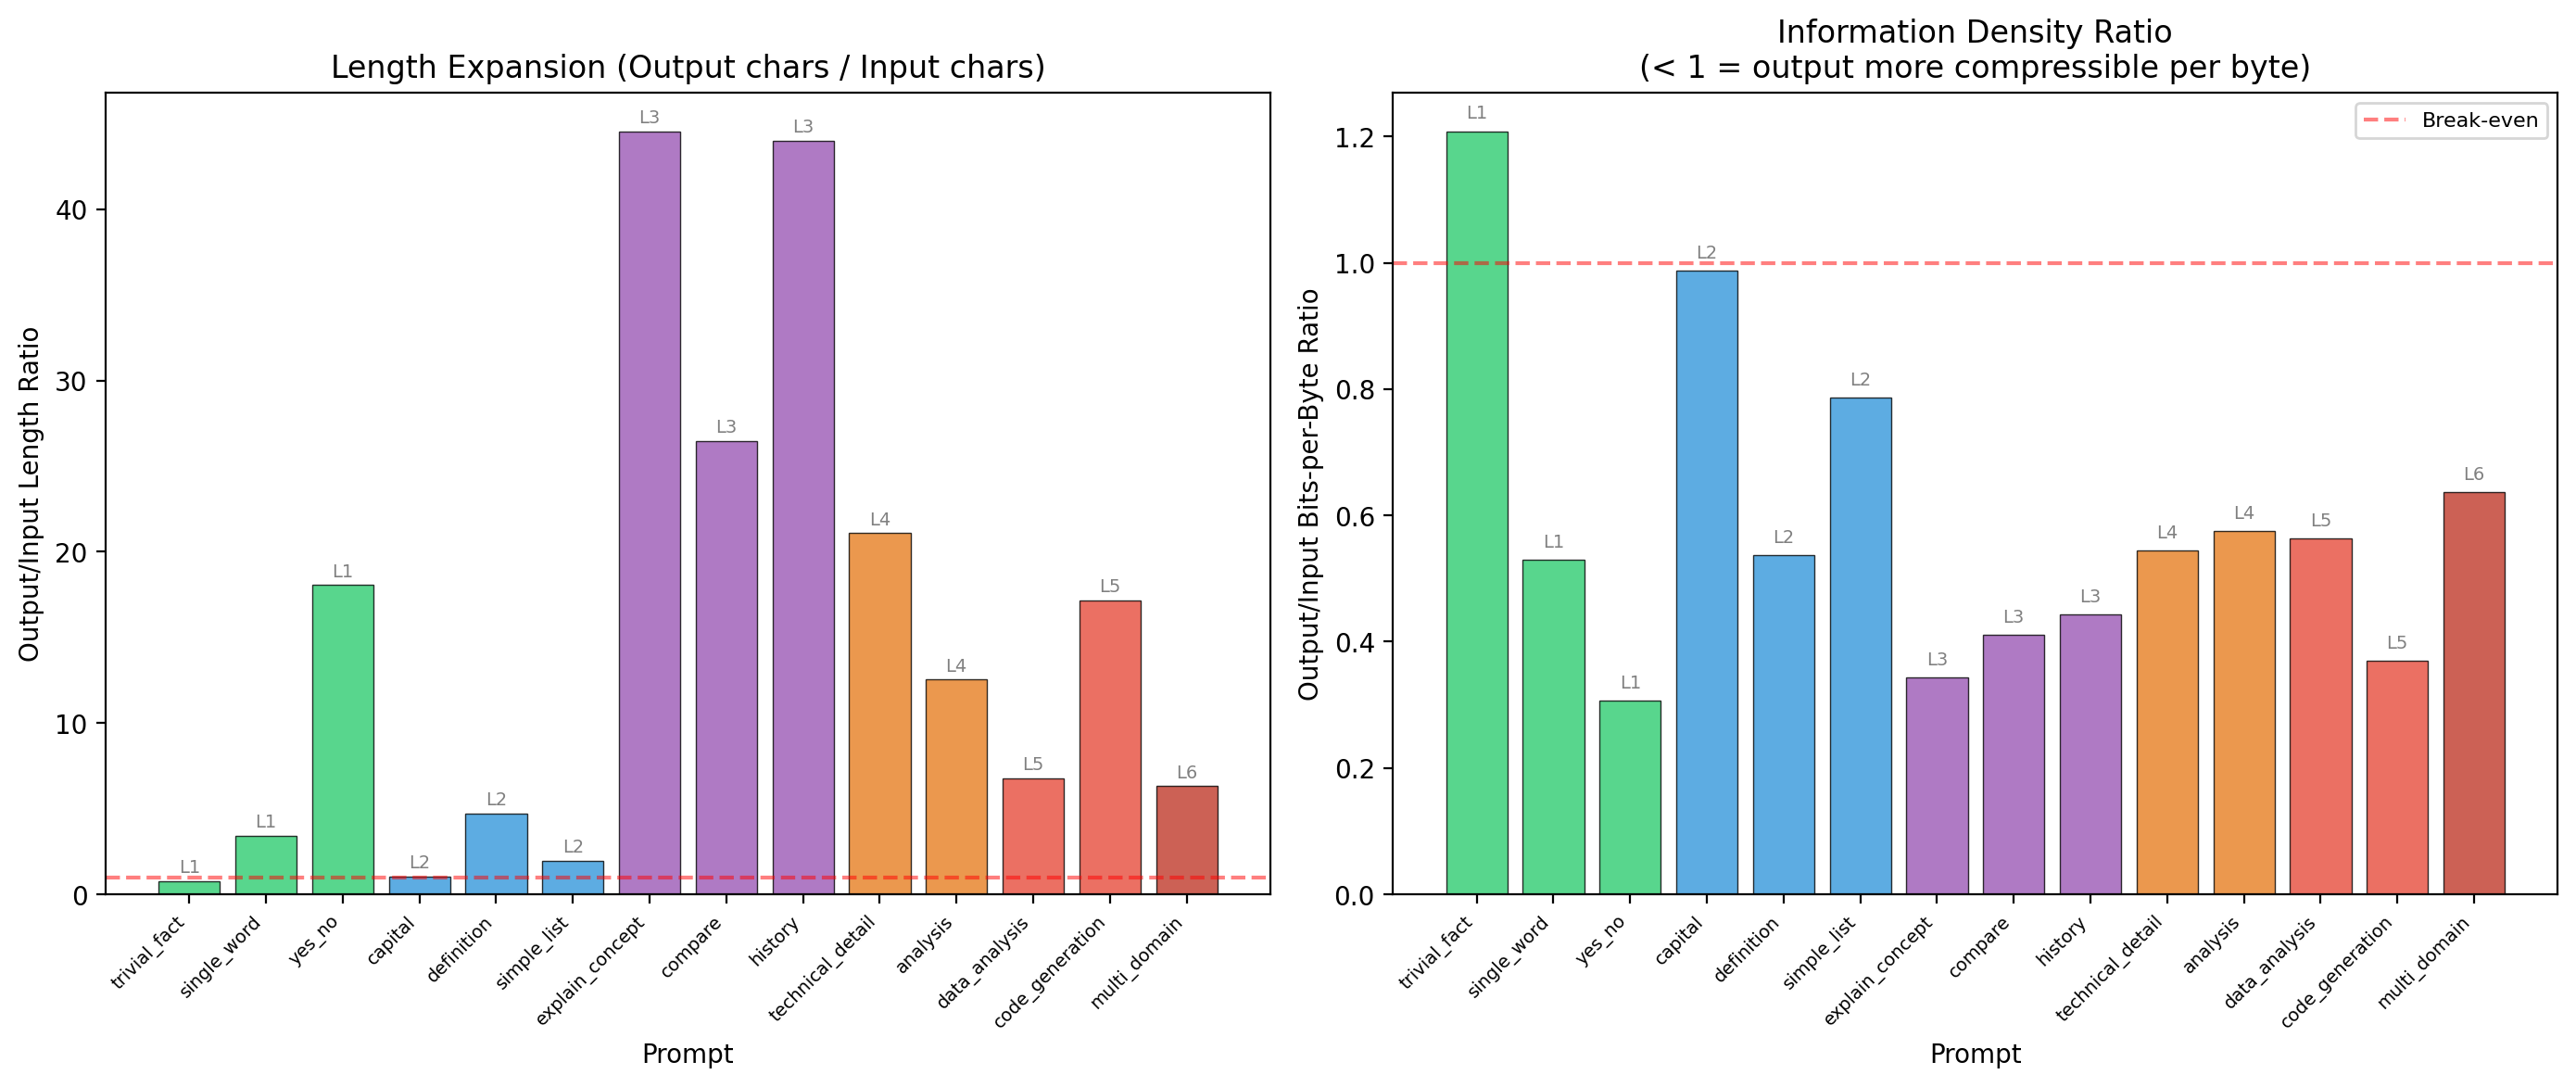
\includegraphics[width=\textwidth]{figures/fig_amplification_decomposition.png}
        \caption{Decomposition of information amplification into length expansion and density ratio. Density ratio is consistently $< 1$.}
        \label{fig:decomp}
    \end{subfigure}
    \caption{Input--output information relationship. \textbf{(a)} Total compressed bits scale linearly with input complexity. \textbf{(b)} The apparent amplification is entirely due to length expansion; per-byte density always decreases.}
    \label{fig:main}
\end{figure}

\begin{figure}[t]
    \centering
    \begin{subfigure}[b]{0.48\textwidth}
        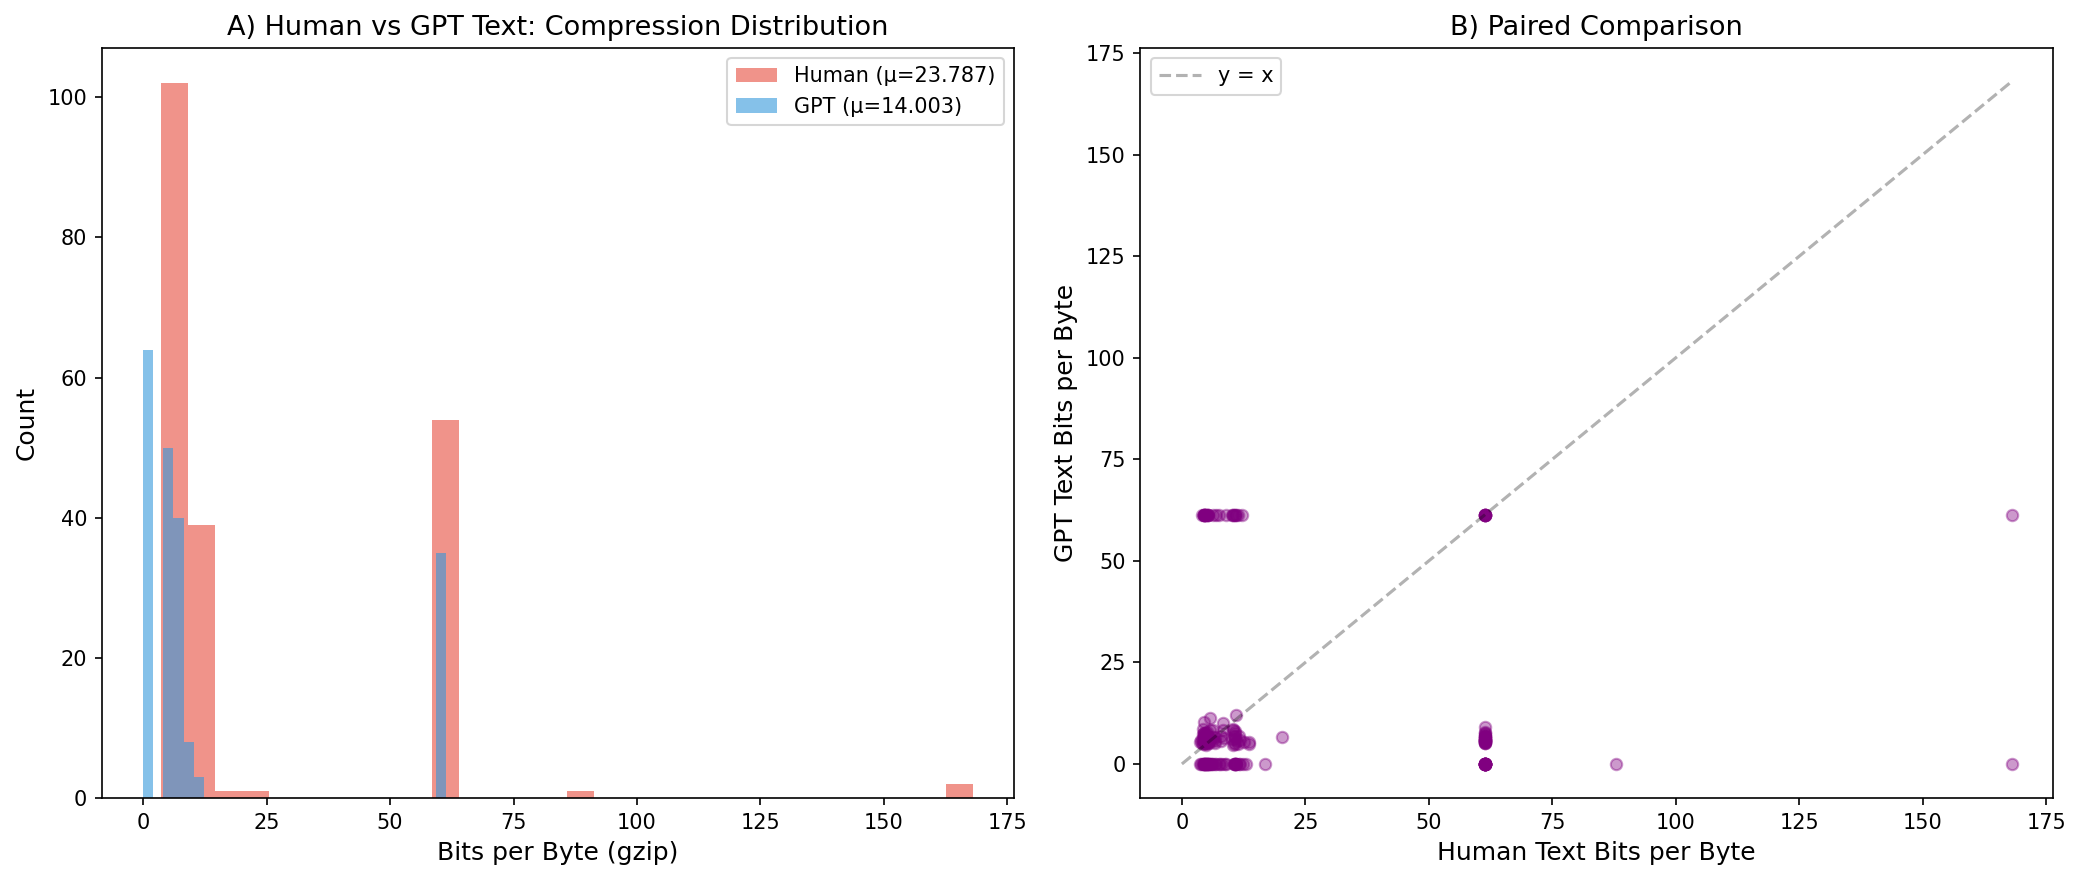
\includegraphics[width=\textwidth]{figures/fig3_human_vs_gpt_compression.png}
        \caption{Human vs.\ GPT text compression by gzip. GPT text is \emph{less} compressible ($p < 10^{-11}$).}
        \label{fig:humanvsgpt}
    \end{subfigure}
    \hfill
    \begin{subfigure}[b]{0.48\textwidth}
        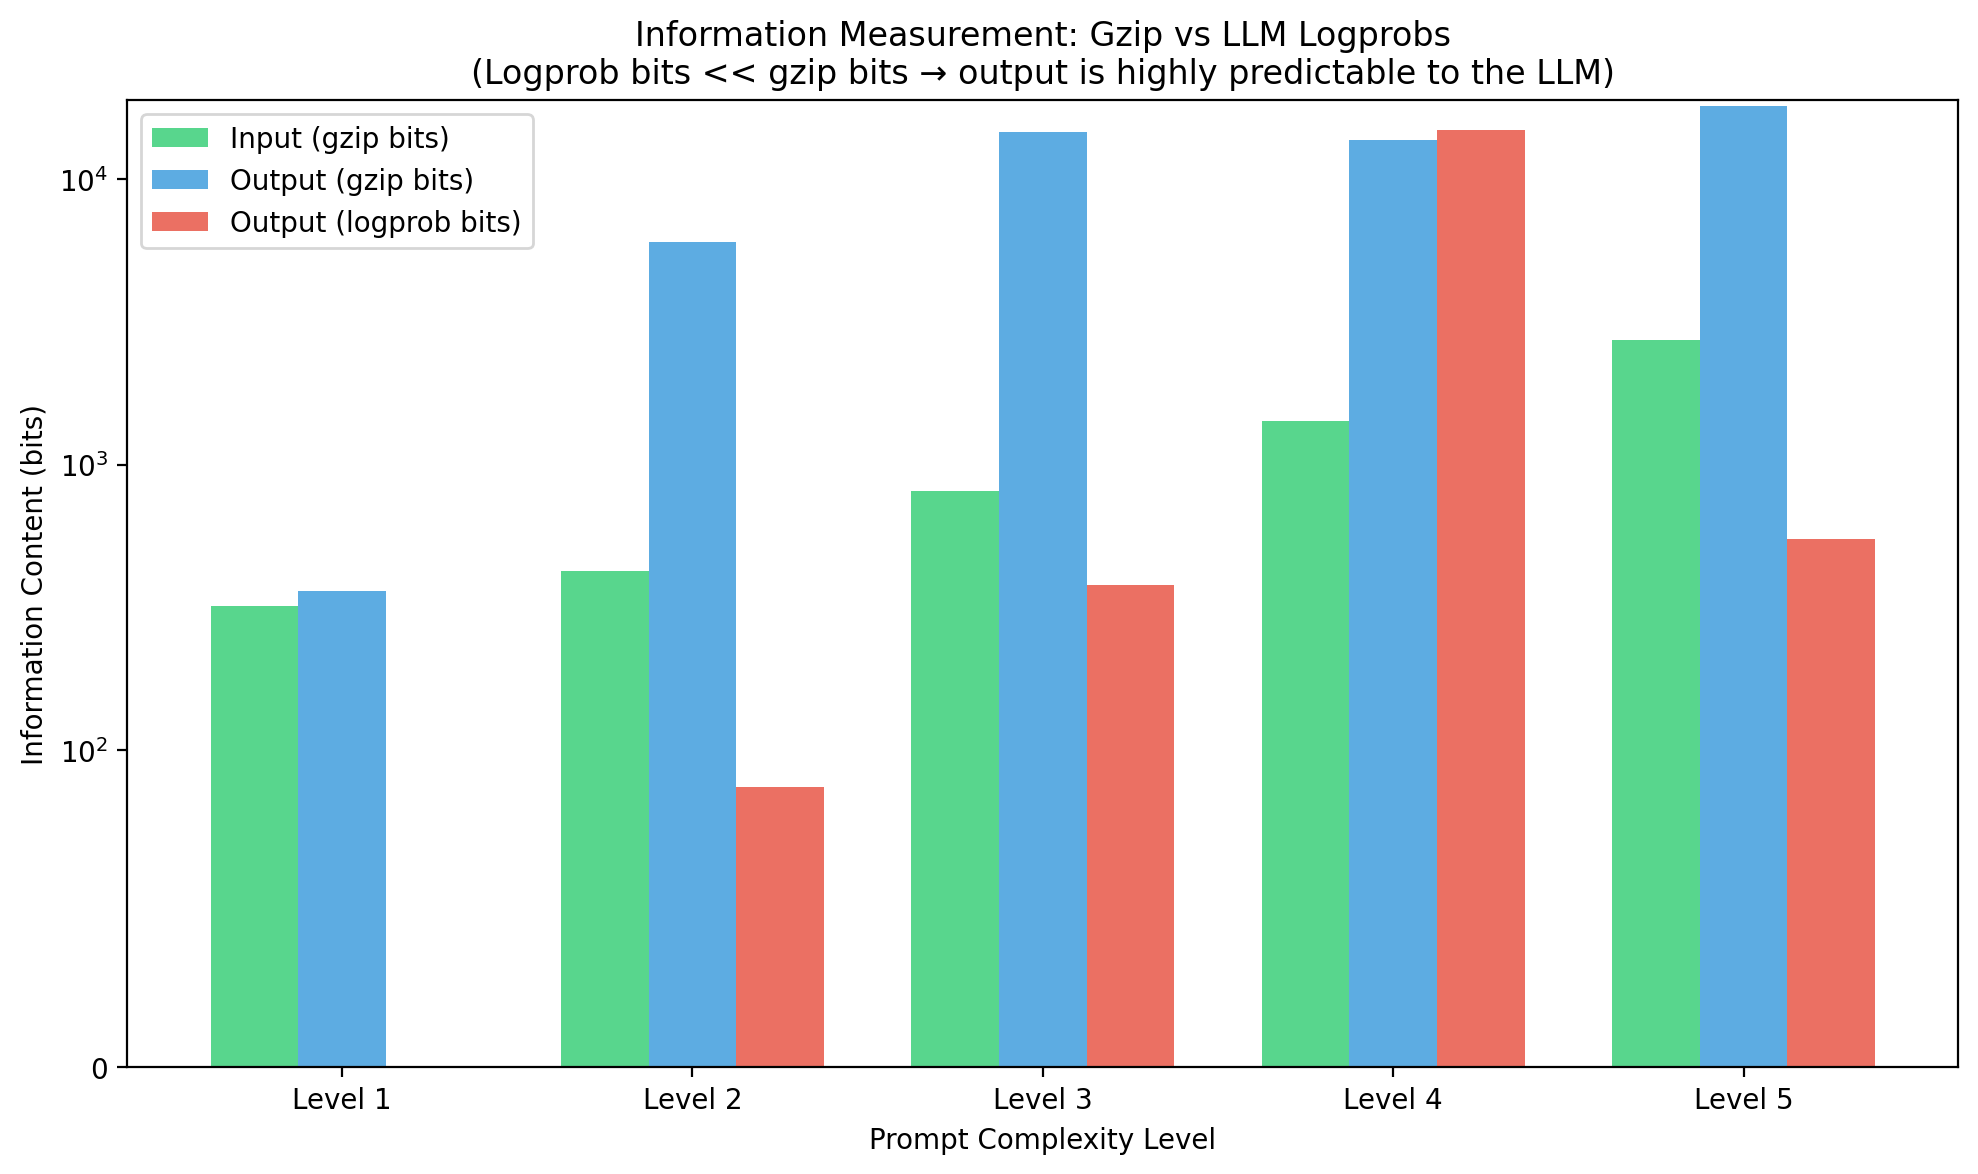
\includegraphics[width=\textwidth]{figures/fig_logprob_vs_gzip.png}
        \caption{Gzip vs.\ log-probability information measures. Log-probabilities assign $10$--$40\times$ fewer bits.}
        \label{fig:logprob}
    \end{subfigure}
    \caption{Compressor dependence. \textbf{(a)} Gzip finds GPT text less compressible than human text---opposite to LLM-based compressors. \textbf{(b)} The model's own log-probabilities reveal that outputs are nearly perfectly predictable.}
    \label{fig:compressor}
\end{figure}
